%\let\cleardoublepage\clearpage
%\chapter*{Appendices} % * means unnumbered heading
%\addcontentsline{toc}{chapter}{Appendices} % add to table of contents although not a numbered heading
%\label{c:Appendices}

\chapter{\ttbar different cross section analysis}
\label{ac:ttbar_diff_cross_section_analysis}

\section{Datasets in differential cross section analysis}
\label{as:datasets}

\begin{table}[hbth]
\centering
\begin{tabular}{lrllr}
\hline
\textbf{Year} & \textbf{\roots} (\TeV) & Channel & \textbf{HLT Trigger} & Run Range \\
\hline
2011 & 7 & electron & HLT\_Ele25\_CaloIdVT\_TrkIdT\_CentralTriJet30 & 160404--163869 \\
2011 & 7 & electron & HLT\_Ele25\_CaloIdVT\_TrkIdT\_TriCentralJet30 & 163870--165633 \\
2011 & 7 & electron & HLT\_Ele25\_CaloIdVT\_CaloIsoT\_TrkIdT\_TrkIsoT\_TriCentralJet30 & 165634--178380 \\
2011 & 7 & electron & HLT\_Ele25\_CaloIdVT\_CaloIsoT\_TrkIdT\_TrkIsoT\_TriCentralPFJet30 & 178381--180252 \\
\hline
2012 & 8 & electron & HLT\_Ele27\_WP80 & all \\
\hline
2011 & 7 & muon & HLT\_IsoMu24 & 160404--160404 \\
2011 & 7 & muon & HLT\_IsoMu24\_eta2p1 & 173236--190456 \\
\hline
2012 & 8 & muon & HLT\_IsoMu24\_eta2p1\_v & all \\
\hline
\end{tabular}
\caption{HLT Triggers used in 2011 and 2012 data in the electron and muon channels.}
\label{tab:HLTTriggers}
\end{table}

% included in main text
%\begin{table}[hbth]
\centering
\begin{tabular}{llrr}
\hline
\textbf{Data set name} & \textbf{Run period} & \textbf{$\mathbf{L_{int}}$ / \pbinv} & \textbf{Runs} \\
\hline
ElectronHad 12 Oct 2013 ReReco & Run2011A & 2,333 & 160404--173692 \\
ElectronHad 12 Oct 2013 ReReco & Run2011B & 2,738 & 175833--180252 \\
\hline
SingleMu 12 Oct 2013 ReReco & Run2011A & 2,331 & 160404--173692 \\
SingleMu 12 Oct 2013 ReReco & Run2011B & 2,766 & 175833--180252 \\
\hline
\end{tabular}
\caption{7 TeV data sets by run period with the corresponding integrated
luminosities ($L_{int}$) and run numbers.}
\label{tab:datasets7TeV}
\end{table}
%\begin{table}[hbth]
\centering
\begin{tabular}{llrr}
\hline
\textbf{Data set name} & \textbf{Run period} & \textbf{$\mathbf{\mathcal{L}_{int}}$ / \pbinv} & \textbf{Runs}
\\
\hline
SingleElectron 22 Jan 2013 ReReco & Run2012A & $883.3$ & 190456--193621 \\
SingleElectron 22 Jan 2013 ReReco & Run2012B & $4,389.0$ & 193834--196531 \\
SingleElectron 22 Jan 2013 ReReco & Run2012C & $7,137.0$ & 198022--203742 \\
SingleElectron 22 Jan 2013 ReReco & Run2012D & $7,318.0$ & 203777--208686 \\
\hline
SingleMu 22 Jan 2013 ReReco & Run2012A & $889.4$ & 190456--193621 \\
SingleMu 22 Jan 2013 ReReco & Run2012B & $4,424.0$ & 193834--196531 \\
SingleMu 22 Jan 2013 ReReco & Run2012C & $7,152.0$ & 198022--203742 \\
SingleMu 22 Jan 2013 ReReco & Run2012D & $7,280.0$ & 203777--208686 \\
\hline
\end{tabular}
\caption{8 TeV data sets by run period with the corresponding integrated
luminosities ($\mathcal{L}_{int}$) and run numbers.}
\label{tab:datasets8TeV}
\end{table}

\begin{table}[hbth]
\centering
\begin{tabular}{lr}
\hline
\textbf{Data Period} & \textbf{Mask} \\
\hline
2011 & \verb|Cert_160404-180252_7TeV_ReRecoNov08_Collisions11_JSON_v2.txt| \\
2012 & \verb|Cert_190456-208686_8TeV_22Jan2013ReReco_Collisions12_JSON.txt| \\
\hline
\end{tabular}
\caption{JSON files used for the 2011 and 2012 data taking periods.}
\label{tab:JSONfiles}
\end{table}

% included in main text
%\begin{table}[hbth]
\centering
\caption{\SI{7}{\TeV} Monte Carlo background datasets used for this analysis. All samples are generated
inclusively if not marked otherwise ($^\star$ generator cut on in-flight-decays of b- and c-hadrons, $^\ominus$ enriched in conversion electrons; $l$ means
all leptonic decays: $l=e,\mu,\tau$; $^\bullet$ generator cut on $m_{Z/\gamma} > 50$~GeV).
\label{tab:backgrounddatasets7TeV}} \small\addtolength{\tabcolsep}{-5pt}
\begin{tabular}{llrrr}
%\multicolumn{6}{c}{Background datasets} 
%\hline
Process & Generator & $\sigma$ ($\pb$) & No. events & \lumiint ($\fbinv$) \\
\hline
\hline
Single \t t-channel ($W\rightarrow l\nu$) & \POWHEG & 64.6 & 3249530 & 50.3 \\
Single \cPaqt t-channel ($W\rightarrow l\nu$) & \POWHEG & 64.6 & 1813615 & 28.1 \\
Single \t s-channel ($W\rightarrow l\nu$) & \POWHEG & 4.21 & 229786 & 54.6 \\
Single \cPaqt s-channel ($W\rightarrow l\nu$) & \POWHEG & 4.21 & 138187 & 32.8 \\
Single \t tW-channel ($W\rightarrow l\nu$) & \POWHEG & 10.6 & 744859 & 70.3 \\
Single \cPaqt tW-channel ($W\rightarrow l\nu$) & \POWHEG & 10.6 & 801626 & 75.6 \\
\hline
W ($\rightarrow l\nu$) + 1 Jet & \MADGRAPH & 4480.0 & 70430949 & 15.7 \\
W ($\rightarrow l\nu$) + 2 Jets & \MADGRAPH & 1435.0 & 25069566 & 17.5 \\
W ($\rightarrow l\nu$) + 3 Jets & \MADGRAPH & 304.2 & 6291772 & 20.7 \\
W ($\rightarrow l\nu$) + 4 Jets & \MADGRAPH & 172.6 & 13240209 & 76.7 \\
$Z$/$\gamma^{*}$ ($\rightarrow l^+l^-$) + jets $^\bullet$ & \MADGRAPH & 3048 & 32846945 & 10.8 \\
\hline
QCD BCtoE \PT 20-30 $^\star$ & \PYTHIA & 139299.0 & 1927944 & 1.4$\times 10^{-2}$ \\
QCD BCtoE \PT 30-80 $^\star$ & \PYTHIA & 143844.8 & 1946505 & 1.4$\times 10^{-2}$ \\
QCD BCtoE \PT 80-170 $^\star$ & \PYTHIA & 9431.1 & 1002427 & 0.1 \\
\hline
QCD EM  \PT 20-30 $^\ominus$ & \PYTHIA & 2502660.0 & 32976415 & 1.3$\times 10^{-2}$ \\ 
QCD EM \PT 30-80 $^\ominus$ & \PYTHIA & 3625840.0 & 71775065 & 2.0$\times 10^{-2}$ \\
QCD EM \PT 80-170 $^\ominus$ & \PYTHIA & 142813.8 & 7650319 & 5.4$\times 10^{-2}$ \\
QCD EM  \PT 170-250 $^\ominus$ & \PYTHIA & 142813.8 & 2968842 & 2.1$\times 10^{-2}$ \\
QCD EM  \PT 250-350 $^\ominus$ & \PYTHIA & 368.0 & 2952960 & 8.0 \\
QCD EM \PT 350-inf $^\ominus$ & \PYTHIA & 55.0 & 2957326 & 53.8 \\
\hline
$\gamma$ + Jets HT 40-100 & \MADGRAPH & 25690.0 & 9882860 & 0.4 \\
$\gamma$ + Jets HT 100-200 & \MADGRAPH & 5213.0 & 1514347 & 0.3 \\
$\gamma$ + Jets HT $>$ 200 & \MADGRAPH & 798.3 & 9275592 & 11.6 \\
\hline
QCD $\mu$ enriched \PT 15-20 & \PYTHIA & 1668096.0 & 1901684 & 1.1$\times 10^{-3}$ \\
QCD $\mu$ enriched \PT 20-30 & \PYTHIA & 1342184.0 & 10173300 & 7.6$\times 10^{-3}$ \\
QCD $\mu$ enriched \PT 30-50 & \PYTHIA & 596506.8 & 11610111 & 1.9$\times 10^{-2}$ \\
QCD $\mu$ enriched \PT 50-80 & \PYTHIA & 140039.55 & 9870031 & 7.0$\times 10^{-2}$ \\
QCD $\mu$ enriched \PT 80-120 & \PYTHIA & 28546.2 & 9769136 & 0.3 \\
QCD $\mu$ enriched \PT 120-170 & \PYTHIA & 4692.91 & 7818474 & 1.7 \\
QCD $\mu$ enriched \PT 170-300 & \PYTHIA & 1445.96 & 8116409 & 5.6 \\
QCD $\mu$ enriched \PT 300-470 & \PYTHIA & 95.4464 & 7870002 & 82.5 \\
QCD $\mu$ enriched \PT 470-600 & \PYTHIA & 7.41697 & 3812529 & 514.0 \\
QCD $\mu$ enriched \PT 600-800 & \PYTHIA & 1.69145 & 4149911 & 2453.5 \\
QCD $\mu$ enriched \PT 800-1000 & \PYTHIA & 0.231869 & 4036867 & 17410.1 \\
QCD $\mu$ enriched \PT 1000-inf & \PYTHIA & 0.053385 & 4133897 & 77435.6 \\
\hline
\end{tabular}
\end{table}
%\begin{table}[hbth]
\centering
\caption{\SI{8}{\TeV} Monte Carlo background datasets used for this analysis. All samples are generated
inclusively if not marked otherwise ($^\star$ generator cut on in-flight-decays of b- and c-hadrons, $^\ominus$ enriched in conversion electrons; $l$ means
all leptonic decays: $l=e,\mu,\tau$; $^\bullet$ generator cut on $m_{Z/\gamma} > 50$~GeV).
\label{tab:backgrounddatasets8TeV}} \small\addtolength{\tabcolsep}{-5pt}
\begin{tabular}{llrrr}
%\multicolumn{6}{c}{Background datasets} 
%\hline
Process & Generator & $\sigma$ ($\pb$) & No. events & \lumiint ($\fbinv$) \\
\hline
\hline
Single \t t-channel ($W\rightarrow l\nu$) & \POWHEG & 55.531 & 3758221 & 67.7 \\
Single \cPaqt t-channel ($W\rightarrow l\nu$) & \POWHEG & 30.0042 & 1906041 & 63.5 \\
Single \t s-channel ($W\rightarrow l\nu$) & \POWHEG & 3.89394 & 259960 & 66.8 \\
Single \cPaqt s-channel ($W\rightarrow l\nu$) & \POWHEG & 1.75776 & 139974 & 79.6 \\
Single \t tW-channel ($W\rightarrow l\nu$) & \POWHEG & 11.1773 & 497657 & 44.5 \\
Single \cPaqt tW-channel ($W\rightarrow l\nu$) & \POWHEG & 11.1773 & 473721 & 42.4 \\
\hline
W ($\rightarrow l\nu$) + 1 Jet & \MADGRAPH & 5400.0 & 23129996 & 15.7 \\
W ($\rightarrow l\nu$) + 2 Jets & \MADGRAPH & 1750.0 & 34027847 & 17.5 \\
W ($\rightarrow l\nu$) + 3 Jets & \MADGRAPH & 519.0 & 15539463 & 20.7 \\
W ($\rightarrow l\nu$) + 4 Jets & \MADGRAPH & 214.0 & 13373865 & 76.7 \\
$Z$/$\gamma^{*}$ ($\rightarrow l^+l^-$) + 1 jet$^\bullet$ & \MADGRAPH & 561.0 & 24032529 & 42.8 \\
$Z$/$\gamma^{*}$ ($\rightarrow l^+l^-$) + 2 jets$^\bullet$ & \MADGRAPH & 181.0 & 21840628 & 0.1 \\
$Z$/$\gamma^{*}$ ($\rightarrow l^+l^-$) + 3 jets$^\bullet$ & \MADGRAPH & 51.1 & 10819603 & 0.2 \\
$Z$/$\gamma^{*}$ ($\rightarrow l^+l^-$) + 4 jets$^\bullet$ & \MADGRAPH & 23.04 & 6381467 & 0.3 \\
\hline
QCD BCtoE \PT 20-30 $^\star$ & \PYTHIA & 167388.0 & 1731522 & 1.0$\times 10^{-2}$ \\
QCD BCtoE \PT 30-80 $^\star$ & \PYTHIA & 167040.0 & 2037907 & 1.2$\times 10^{-2}$ \\
QCD BCtoE \PT 80-170 $^\star$ & \PYTHIA & 12981.9 & 1945523 & 0.1 \\
QCD BCtoE \PT 170-250 $^\star$ & \PYTHIA & 632.0 & 1948112 & 3.1 \\
QCD BCtoE \PT 250-350 $^\star$ & \PYTHIA & 103.3 & 2026516 & 19.6 \\
QCD BCtoE \PT 350-inf $^\star$ & \PYTHIA & 23.9 & 1948525 & 81.5 \\
\hline
QCD EM  \PT 20-30 $^\ominus$ & \PYTHIA & 2914860.0 & 34830398 & 1.2$\times 10^{-2}$ \\ 
QCD EM \PT 30-80 $^\ominus$ & \PYTHIA & 4615893.0 & 32443607 & 7.0$\times 10^{-3}$ \\
QCD EM \PT 80-170 $^\ominus$ & \PYTHIA & 183294.9 & 34024542 & 0.2 \\
QCD EM  \PT 170-250 $^\ominus$ & \PYTHIA & 4586.5 & 31696985 & 6.9 \\
QCD EM  \PT 250-350 $^\ominus$ & \PYTHIA & 556.7 & 33659467 & 60.5 \\
QCD EM \PT 350-inf $^\ominus$ & \PYTHIA & 89.1 & 33756727 & 378.8 \\
\hline
$\gamma$ + Jets HT 200-400 & \MADGRAPH & 960.5 & 47316433 & 49.3 \\
$\gamma$ + Jets HT 400-inf & \MADGRAPH & 107.5 & 9491846 & 88.3 \\
\hline
QCD $\mu$ enriched \PT 15-20 & \PYTHIA & 2738580.0 & 1722678 & 0.6$\times 10^{-3}$ \\
QCD $\mu$ enriched \PT 20-30 & \PYTHIA & 1865500.0 & 8486893 & 4.5$\times 10^{-3}$ \\
QCD $\mu$ enriched \PT 30-50 & \PYTHIA & 806298.0 & 9560248 & 1.2$\times 10^{-2}$ \\
QCD $\mu$ enriched \PT 50-80 & \PYTHIA & 176187.6 & 10365209 & 5.9$\times 10^{-2}$ \\
QCD $\mu$ enriched \PT 80-120 & \PYTHIA & 40448.0 & 9238622 & 0.2 \\
QCD $\mu$ enriched \PT 120-170 & \PYTHIA & 7463.94 & 8501920 & 1.1 \\
QCD $\mu$ enriched \PT 170-300 & \PYTHIA & 2299.752 & 7669932 & 3.3 \\
QCD $\mu$ enriched \PT 300-470 & \PYTHIA & 151.8048 & 7832248 & 51.6 \\
QCD $\mu$ enriched \PT 470-600 & \PYTHIA & 11.79648 & 3783066 & 320.7 \\
QCD $\mu$ enriched \PT 600-800 & \PYTHIA & 2.690196 & 4118988 & 1531.1 \\
QCD $\mu$ enriched \PT 800-1000 & \PYTHIA & 0.3687810 & 4099633 & 11116.7 \\
QCD $\mu$ enriched \PT 1000-inf & \PYTHIA & 0.0849078 & 9238622 & 108807.7 \\
\hline
\end{tabular}
\end{table}


\section{Data - Monte Carlo corrections}
\label{as:data_monte_carlo_corrections}
\begin{figure}[hbtp]
    \centering
      \includegraphics[width=0.48\textwidth]{Chapters/04_Analysis/04b_XSections/images/control_plots/before_fit/7TeV/EPlusJets_nVertex__with_ratio}\hfill
      \includegraphics[width=0.48\textwidth]{Chapters/04_Analysis/04b_XSections/images/control_plots/before_fit/7TeV/EPlusJets_nVertex_reweighted__with_ratio}\\
      \includegraphics[width=0.48\textwidth]{Chapters/04_Analysis/04b_XSections/images/control_plots/before_fit/8TeV/EPlusJets_nVertex__with_ratio}\hfill
      \includegraphics[width=0.48\textwidth]{Chapters/04_Analysis/04b_XSections/images/control_plots/before_fit/8TeV/EPlusJets_nVertex_reweighted__with_ratio}\\
     \caption[Distributions of the number of reconstructed vertices in an event in the muon+jets channel
     before and after implementing pileup reweighting at $\roots=7\TeV$ and $\roots=8\TeV$.]{Distributions of
     the number of reconstructed vertices in an event in the muon+jets channel before implementing pileup
     reweighting (left) and after implementation (right) at $\roots=7\TeV$ (upper) and $\roots=8\TeV$ (lower).}
     \label{fig:nvertices_before_and_after_pileup_reweighting_muons}
\end{figure}

\begin{figure}[hbtp]
    \centering
      \includegraphics[width=0.48\textwidth]{Chapters/04_Analysis/04b_XSections/images/control_plots/before_fit/7TeV/MuPlusJets_N_BJets_with_ratio}\hfill
      \includegraphics[width=0.48\textwidth]{Chapters/04_Analysis/04b_XSections/images/control_plots/before_fit/7TeV/MuPlusJets_N_BJets_reweighted_with_ratio}\\
      \includegraphics[width=0.48\textwidth]{Chapters/04_Analysis/04b_XSections/images/control_plots/before_fit/8TeV/MuPlusJets_N_BJets_with_ratio}\hfill
      \includegraphics[width=0.48\textwidth]{Chapters/04_Analysis/04b_XSections/images/control_plots/before_fit/8TeV/MuPlusJets_N_BJets_reweighted_with_ratio}\\
     \caption[Distributions of the number of \btags in an event in the muon+jets channel before
     and after applying \btag scale factors at $\roots=7\TeV$ and $\roots=8\TeV$.]{Distributions of
     the number of \btags in an event in the muon+jets channel before applying \btag scale factors (left) and
     after application (right) at $\roots=7\TeV$ (upper) and $\roots=8\TeV$ (lower).}
     \label{fig:nbjets_before_and_after_btag_scale_factors_muons}
\end{figure}

\begin{figure}[hbtp]
    \centering
      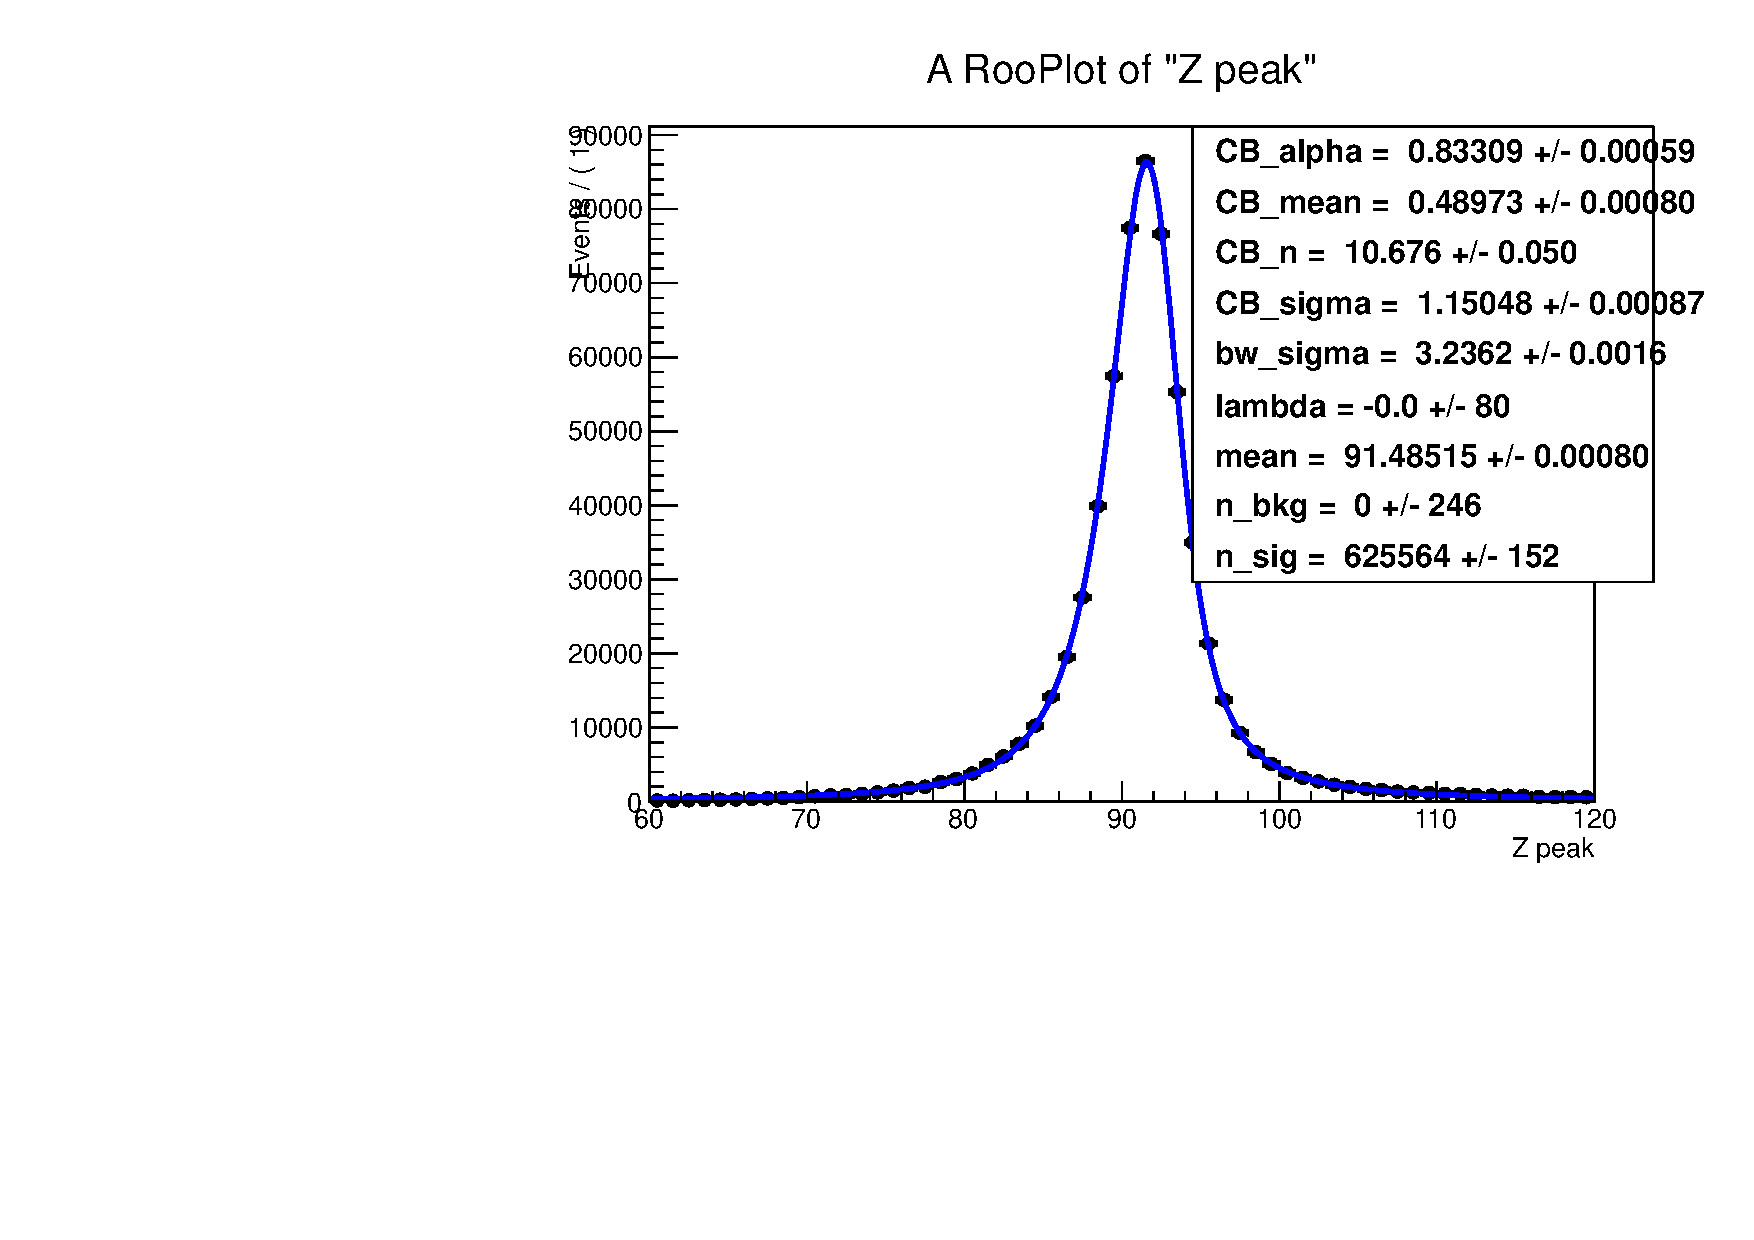
\includegraphics[width=0.48\textwidth]{Chapters/04_Analysis/04b_XSections/images/lepton_scale_factors/CBConvolution/electron/data/trigger/tagProbe_total_Z_peak}\hfill
      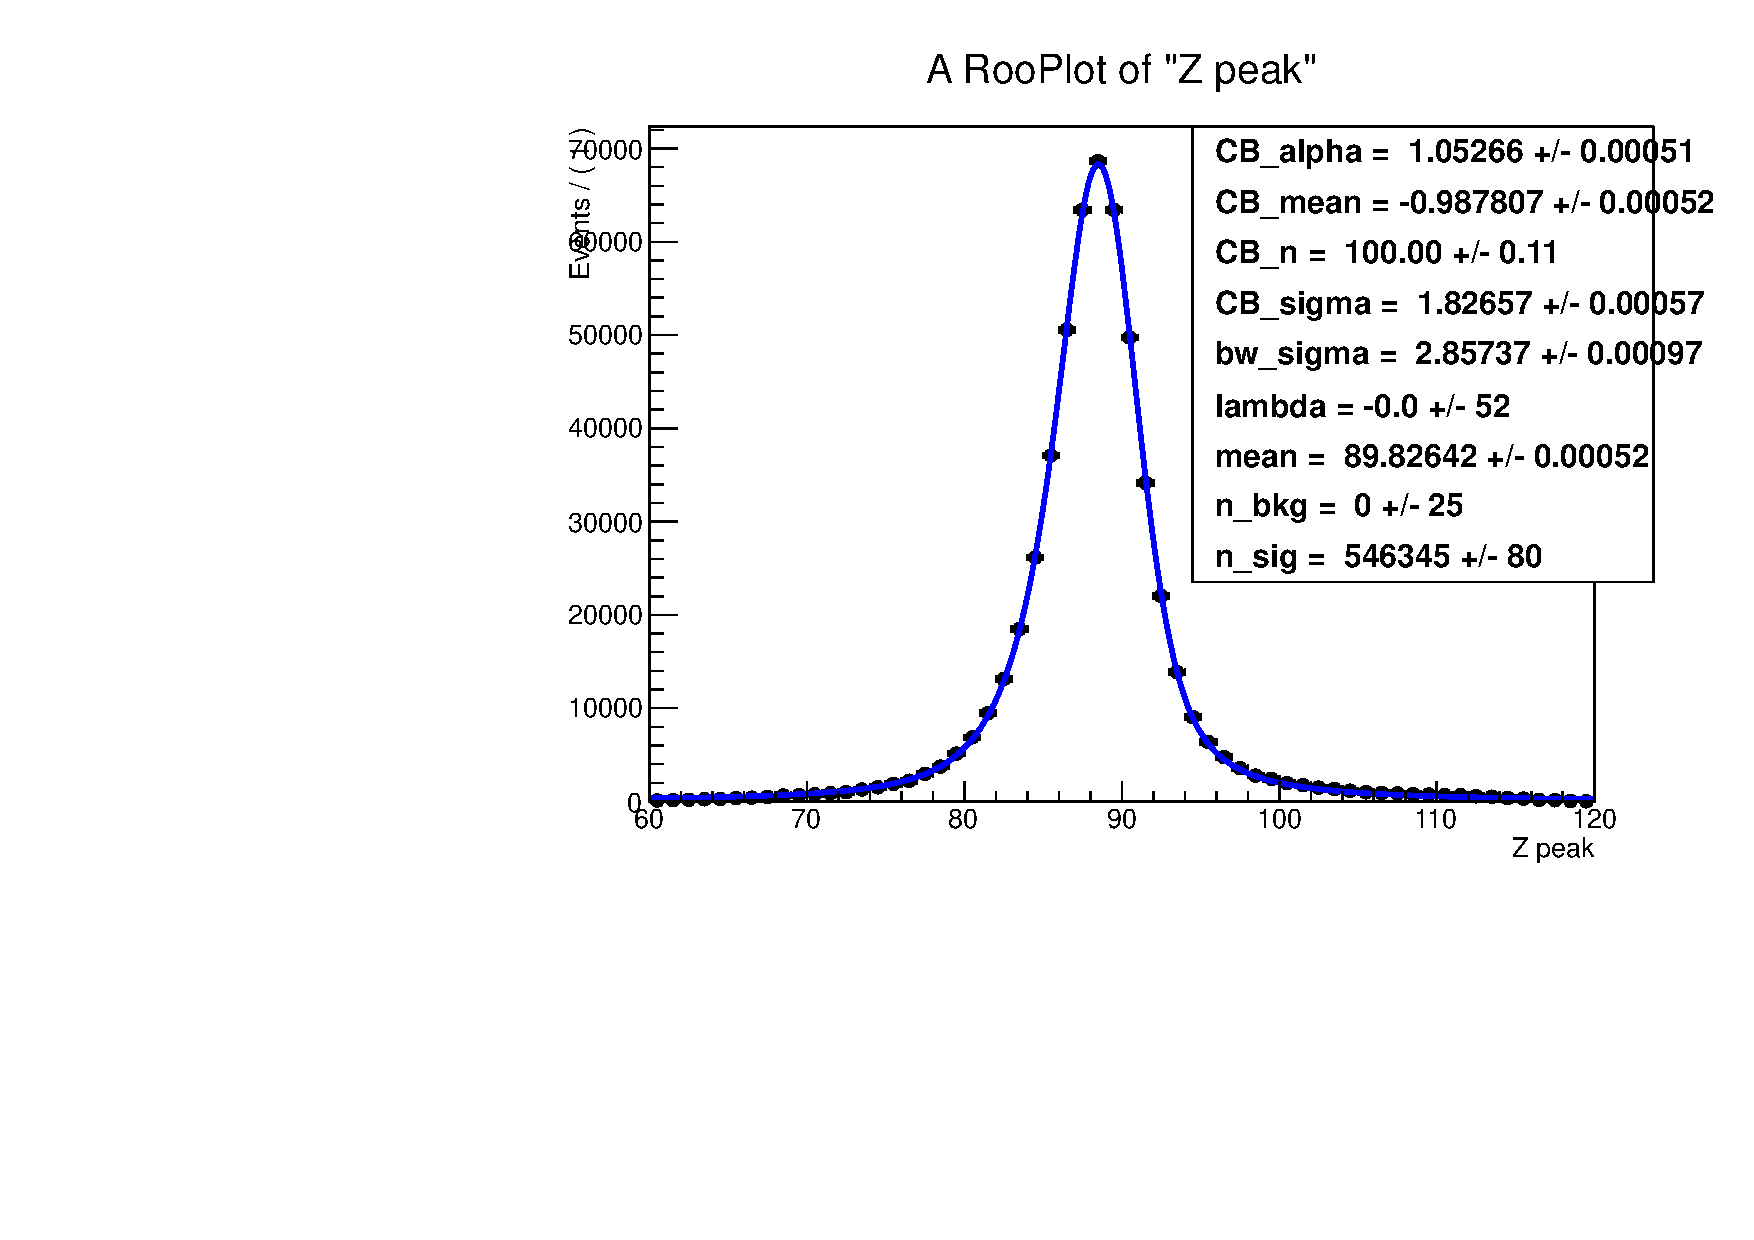
\includegraphics[width=0.48\textwidth]{Chapters/04_Analysis/04b_XSections/images/lepton_scale_factors/CBConvolution/electron/data/trigger/tagProbe_passed_hlt_Z_peak}\\
     \caption[Fits of the invariant mass distribution of tag-and-probe electron pairs.]{Fits of the
     invariant mass distribution of all tag-and-probe pairs (left) and for tag-and-probe pairs in which the
     probe passes the trigger (right).}
     \label{fig:electron_trigger_efficiency_invariant_Z_mass_fits}
\end{figure}

\begin{figure}[hbtp]
    \centering
      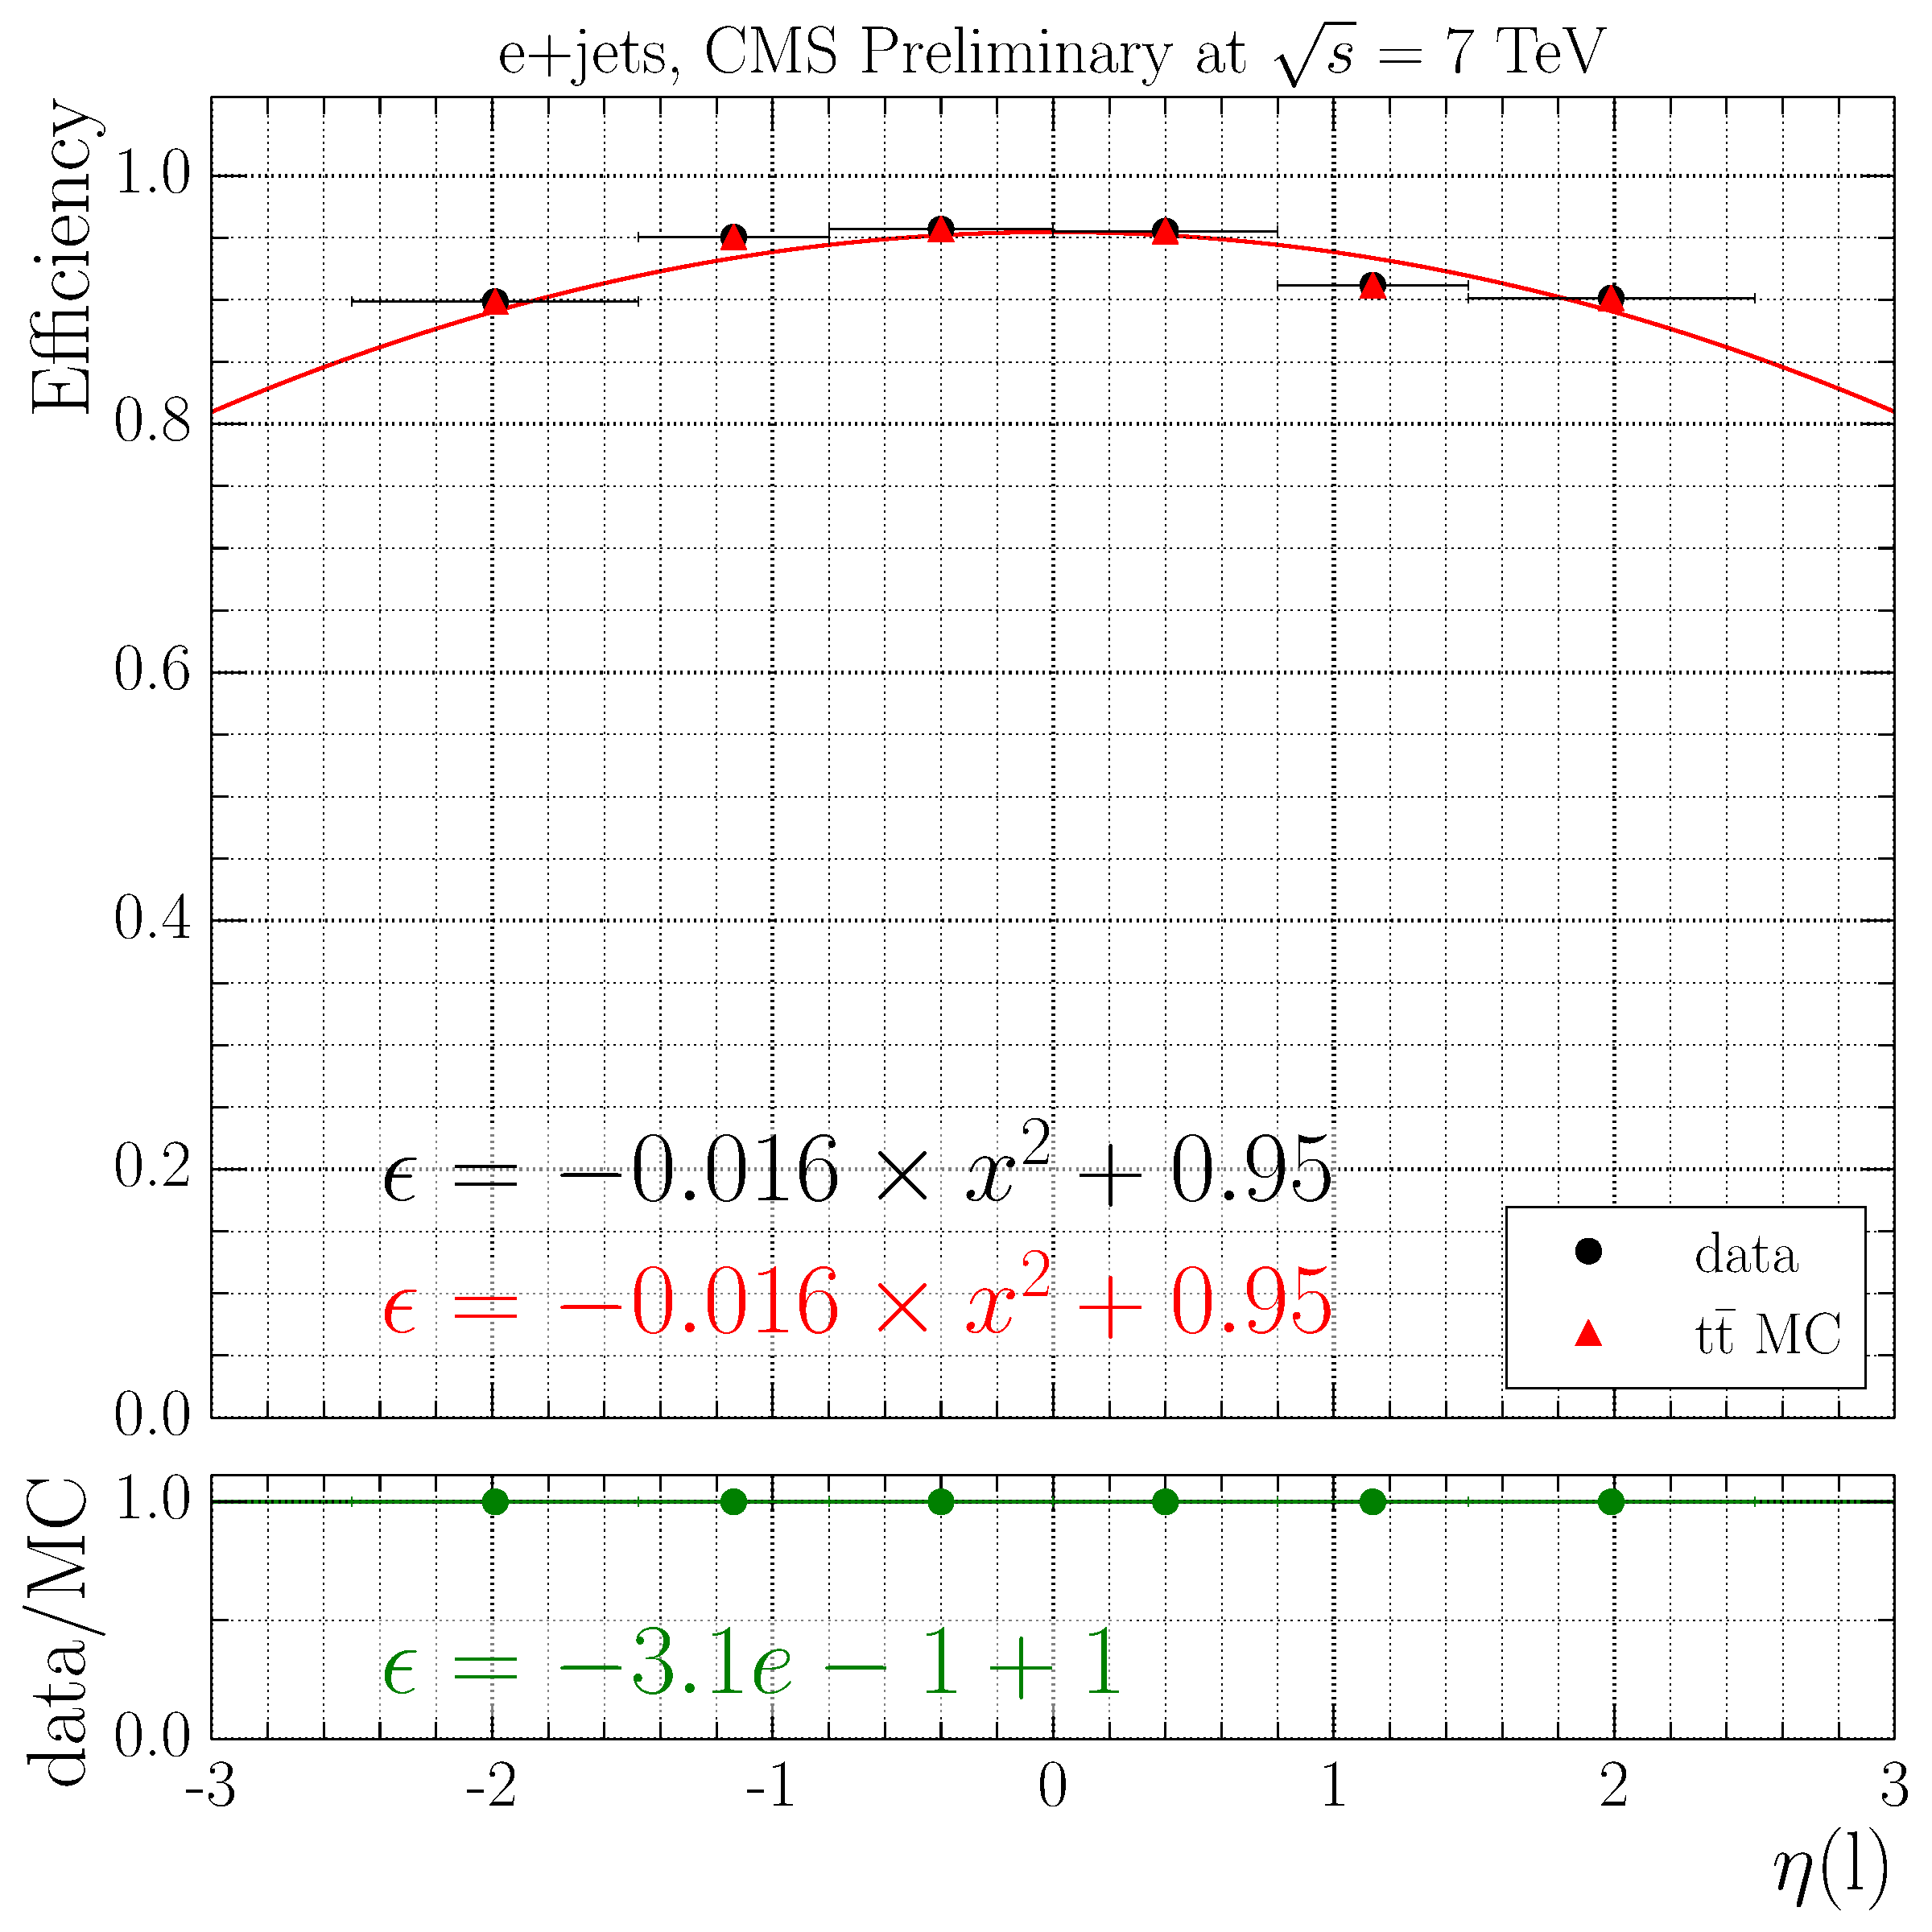
\includegraphics[width=0.48\textwidth]{Chapters/04_Analysis/04b_XSections/images/lepton_scale_factors/CBConvolution/electron/efficiency_eta_trigger}\hfill
      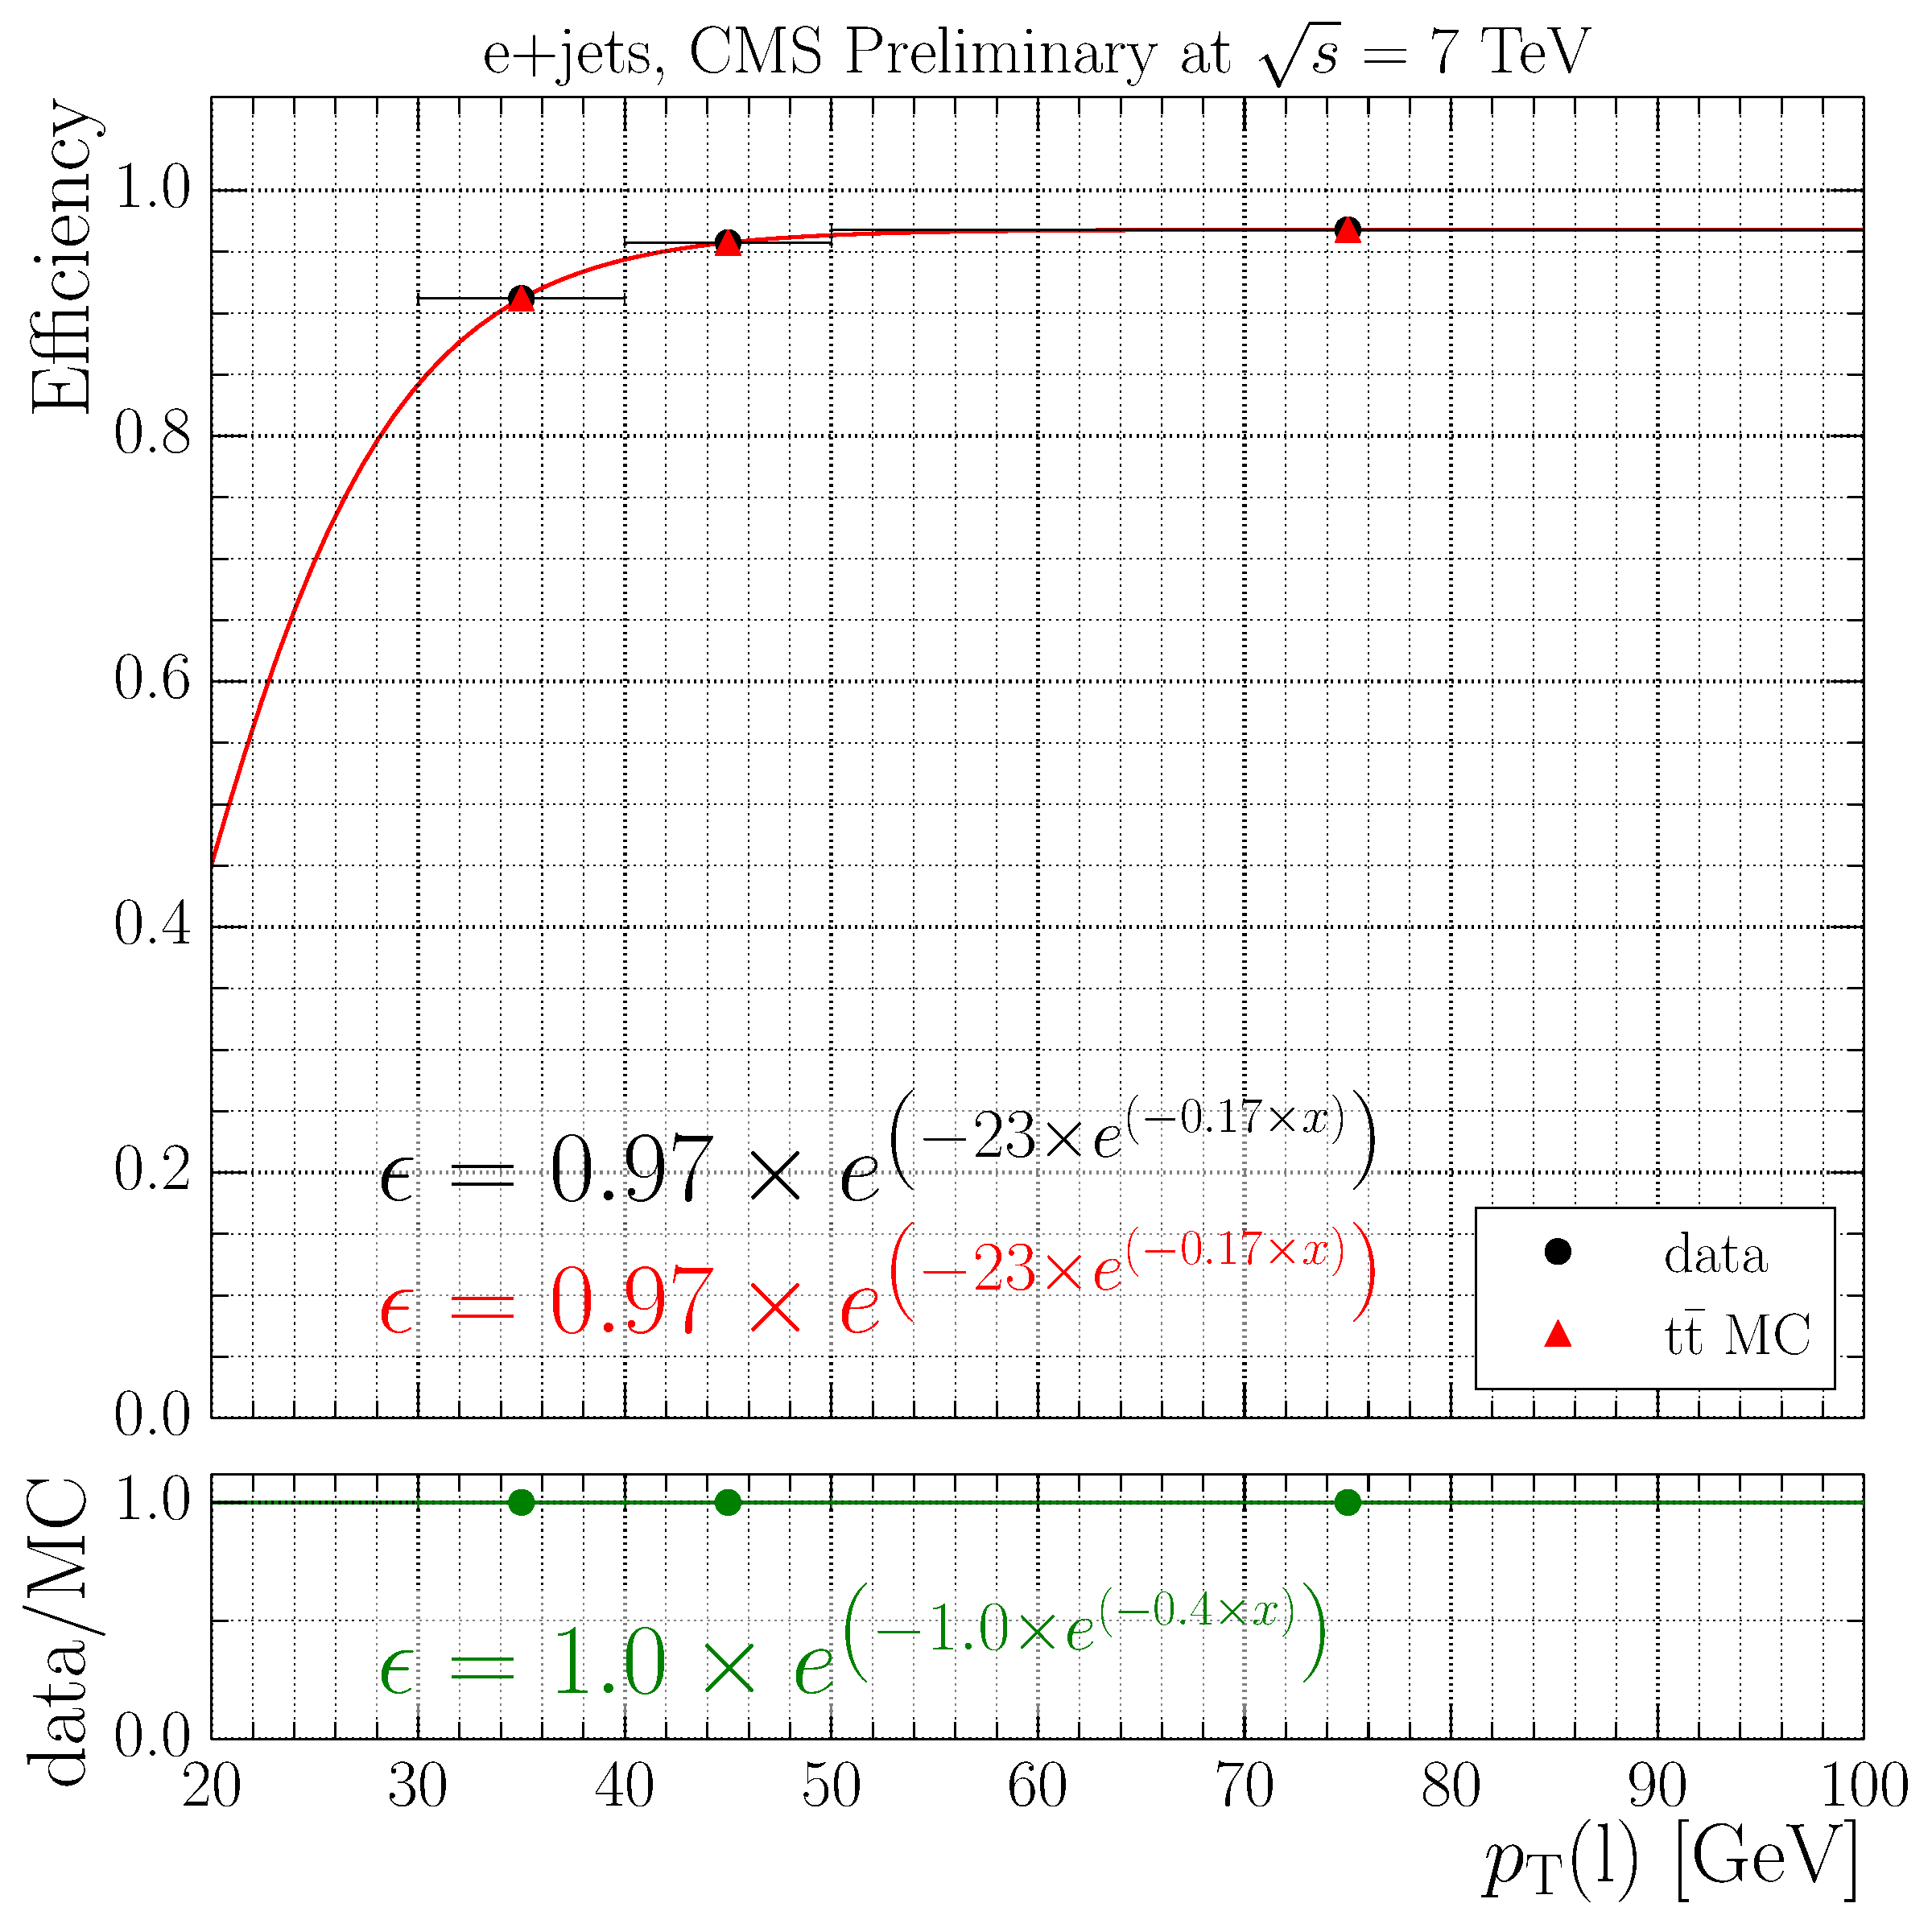
\includegraphics[width=0.48\textwidth]{Chapters/04_Analysis/04b_XSections/images/lepton_scale_factors/CBConvolution/electron/efficiency_pt_trigger}\\
      \caption[Trigger efficiencies as a function of $\eta$ and \pt in data and \ttbar Monte Carlo
      simulation.]{Trigger efficiencies as a function of $\eta$ and \pt in data and \ttbar Monte Carlo
      simulation.}
     \label{fig:electron_trigger_efficiencies_wrt_eta_pt}
\end{figure}
